\chapter*{Introduction}\label{Introduction}
\addcontentsline{toc}{chapter}{Introduction}

The era of geographical explorations of the Earth ended in the past century. 
Mount Everest was  climbed in 1953, the Mariana Trench descended in 1960 and the North and South  Poles reached around 1908 and in 1911, respectively.
The past century will be remembered for an even more important milestone: we understood the structure of everyday matter, and in particular quantum mechanics and relativity have taught us that often the `stuff' that we observe has a intrinsic nature that differs from our intuition.
Does that mean that the age of scientific explorations of matter is over? 
Not yet.
There is more matter left to be understood. In fact, the bulk of the matter in the Universe is not yet understood  and goes by the name of Dark Matter (DM).

In a similar way as the geographical explorations have turned from Earth to space, so have our explorations of matter. 
The existence of DM is established by observations from galactic to cosmological scales.
However, these observations only probe the gravitational coupling of DM --- the total mass and its spatial distributions.
In order to understand what DM truly is, 
we also need to observe its other possible interactions with ordinary matter.

Given the importance of the problem it is not surprising that the subject of DM has attracted a lot of attention:
many experiments are being performed (see fig.\fig{worldplot}), and
presently about 10\% of the papers in cosmology, astrophysics and 
particle physics mention `dark matter'. 
Among others, several reviews about DM, with different scopes and thrusts, have been written in the past~\cite{otherpastDMreviews}.



\begin{table}[b]
\begin{center}\color{black}
\parbox{0.75\textwidth}{\fboxrule=3pt
\centering{\fbox{\fbox{\Huge\bf DARK MATTER}}} \\
\medskip
\centering{$\bullet~\bullet~\bullet$~Needs confirmation~$\bullet~\bullet~\bullet$} \\
\medskip
\hrule height 2pt
\medskip\centerline{\Large\bf PROPERTIES}
\begin{tabular}{ccccc}
\small  $I (J^{PC}) $ & \small MASS &\small  WIDTH & \small DECAY MODES & \small PRODUCTION\\ \hline
 $?(?^{??})$& ${?} \pm {?}$ & ${?} \pm {?}$ &  STABLE ? &   $\sigma({??}\to {??})={?}$
\end{tabular}
\hrule height 2pt}
\end{center}
\caption[DM summary]{\em Summary of currently known Dark Matter properties.  \label{tab:DMsummary}}
\end{table}


This brings us to the question: why another review? 
The reason, at least from our standpoint, is that the field has experienced a rapid evolution in the past years, and is now at a turning point. For example, not so many years ago the term `neutralino' was often used as synonymous with `WIMP'
(Weakly Interacting Massive Particle), which in turn was used interchangeably with `DM particle', and hence simply `DM'. 
As we will discuss at length in the review, and as is obvious to those working in the field, 
these are drastic and narrow simplifications. 
They were somewhat  justified by the theoretical prejudices that dominated 
the field of particle physics up to about a decade ago, but they are no longer justified nowadays. 
The rethinking of those theoretical assumptions was triggered by the fact that 
the very theoretical basis of the neutralinos --- supersymmetry ---
did not show up at colliders, where experimental searches made significant progress after the start of the Large Hadron Collider, with no positive evidence so far.
Furthermore, the WIMP hypothesis itself is under close scrutiny, and has had the viable parameter space reduced significantly over the past two decades. Even the once common implicit assumption that the DM is a new elementary particle is now being reconsidered.

The lack of experimental evidence for non-gravitational interactions of DM may suggest that Dark Matter is something beyond our current theoretical paradigms
and the community is exploring possibilities which received less attention so far.

At this point in time it thus seems useful to review the status of DM research, from a broader point of view. 
This does not mean dismissing the `traditional' research directions but rather adding new ones.
The challenge one faces in doing so is that the field is fragmenting, 
making it difficult to decide to which topics or aspects one should give more weight in such an endeavour. 
The current situation in physics of DM might be similar to the point in time when ancient philosophers were discussing the nature of ordinary matter:
the vague idea of atoms was proposed together with other possibilities,
good ideas accumulated until the discussions stalled,
waiting for the `eureka' moment, after which a coherent picture emerged and sensible results accumulated.
Table~\ref{tab:DMsummary} summarizes the current status, and
fig.\fig{ScientificProgressPlot} shows the typical learning curve of science.

\begin{figure}[t]
$$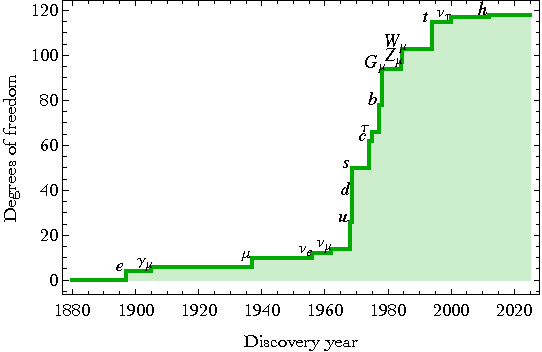
\includegraphics[width=0.47\textwidth]{figs/ParticleProgressPlot}\qquad
\raisebox{1.5ex}{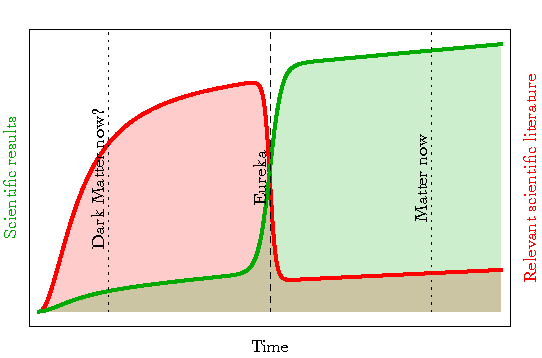
\includegraphics[width=0.48\textwidth]{figs/ScientificProgressPlot}}$$
\caption[Scientific progress]{\em {\bfseries Left:} discovery year of particles.
{\bfseries Right:} typical behaviour of scientific progress.
The field of DM research is nowadays ahead of its `eureka' (discovery) moment: a vast scientific literature discusses
the many open possibilities, on the basis of relatively few solid results. After that moment, hypotheses will drastically shrink and more measurements will flow.
 \label{fig:ScientificProgressPlot}  }
\end{figure}

\medskip

Fig.\fig{DMpapers} shows the map of recent literature: Dark Matter is at the interface between
high-energy experiment, high energy phenomenology, astrophysics, and cosmology, 
where no paper about DM emerges as the one completely dominating the citation counts.
Writing a review about DM in this time and age thus somewhat resembles the problem of summarizing a soccer match with a partial $0-0$ score, where
one can easily fall into a trap of compiling a boring list of various attempts. 
We hope we succeeded in striking instead a reasonable balance between a brief discussion 
of the main points of the various possibilities and a comprehensive but tedious catalogue.

\medskip



\begin{figure}[t]
$$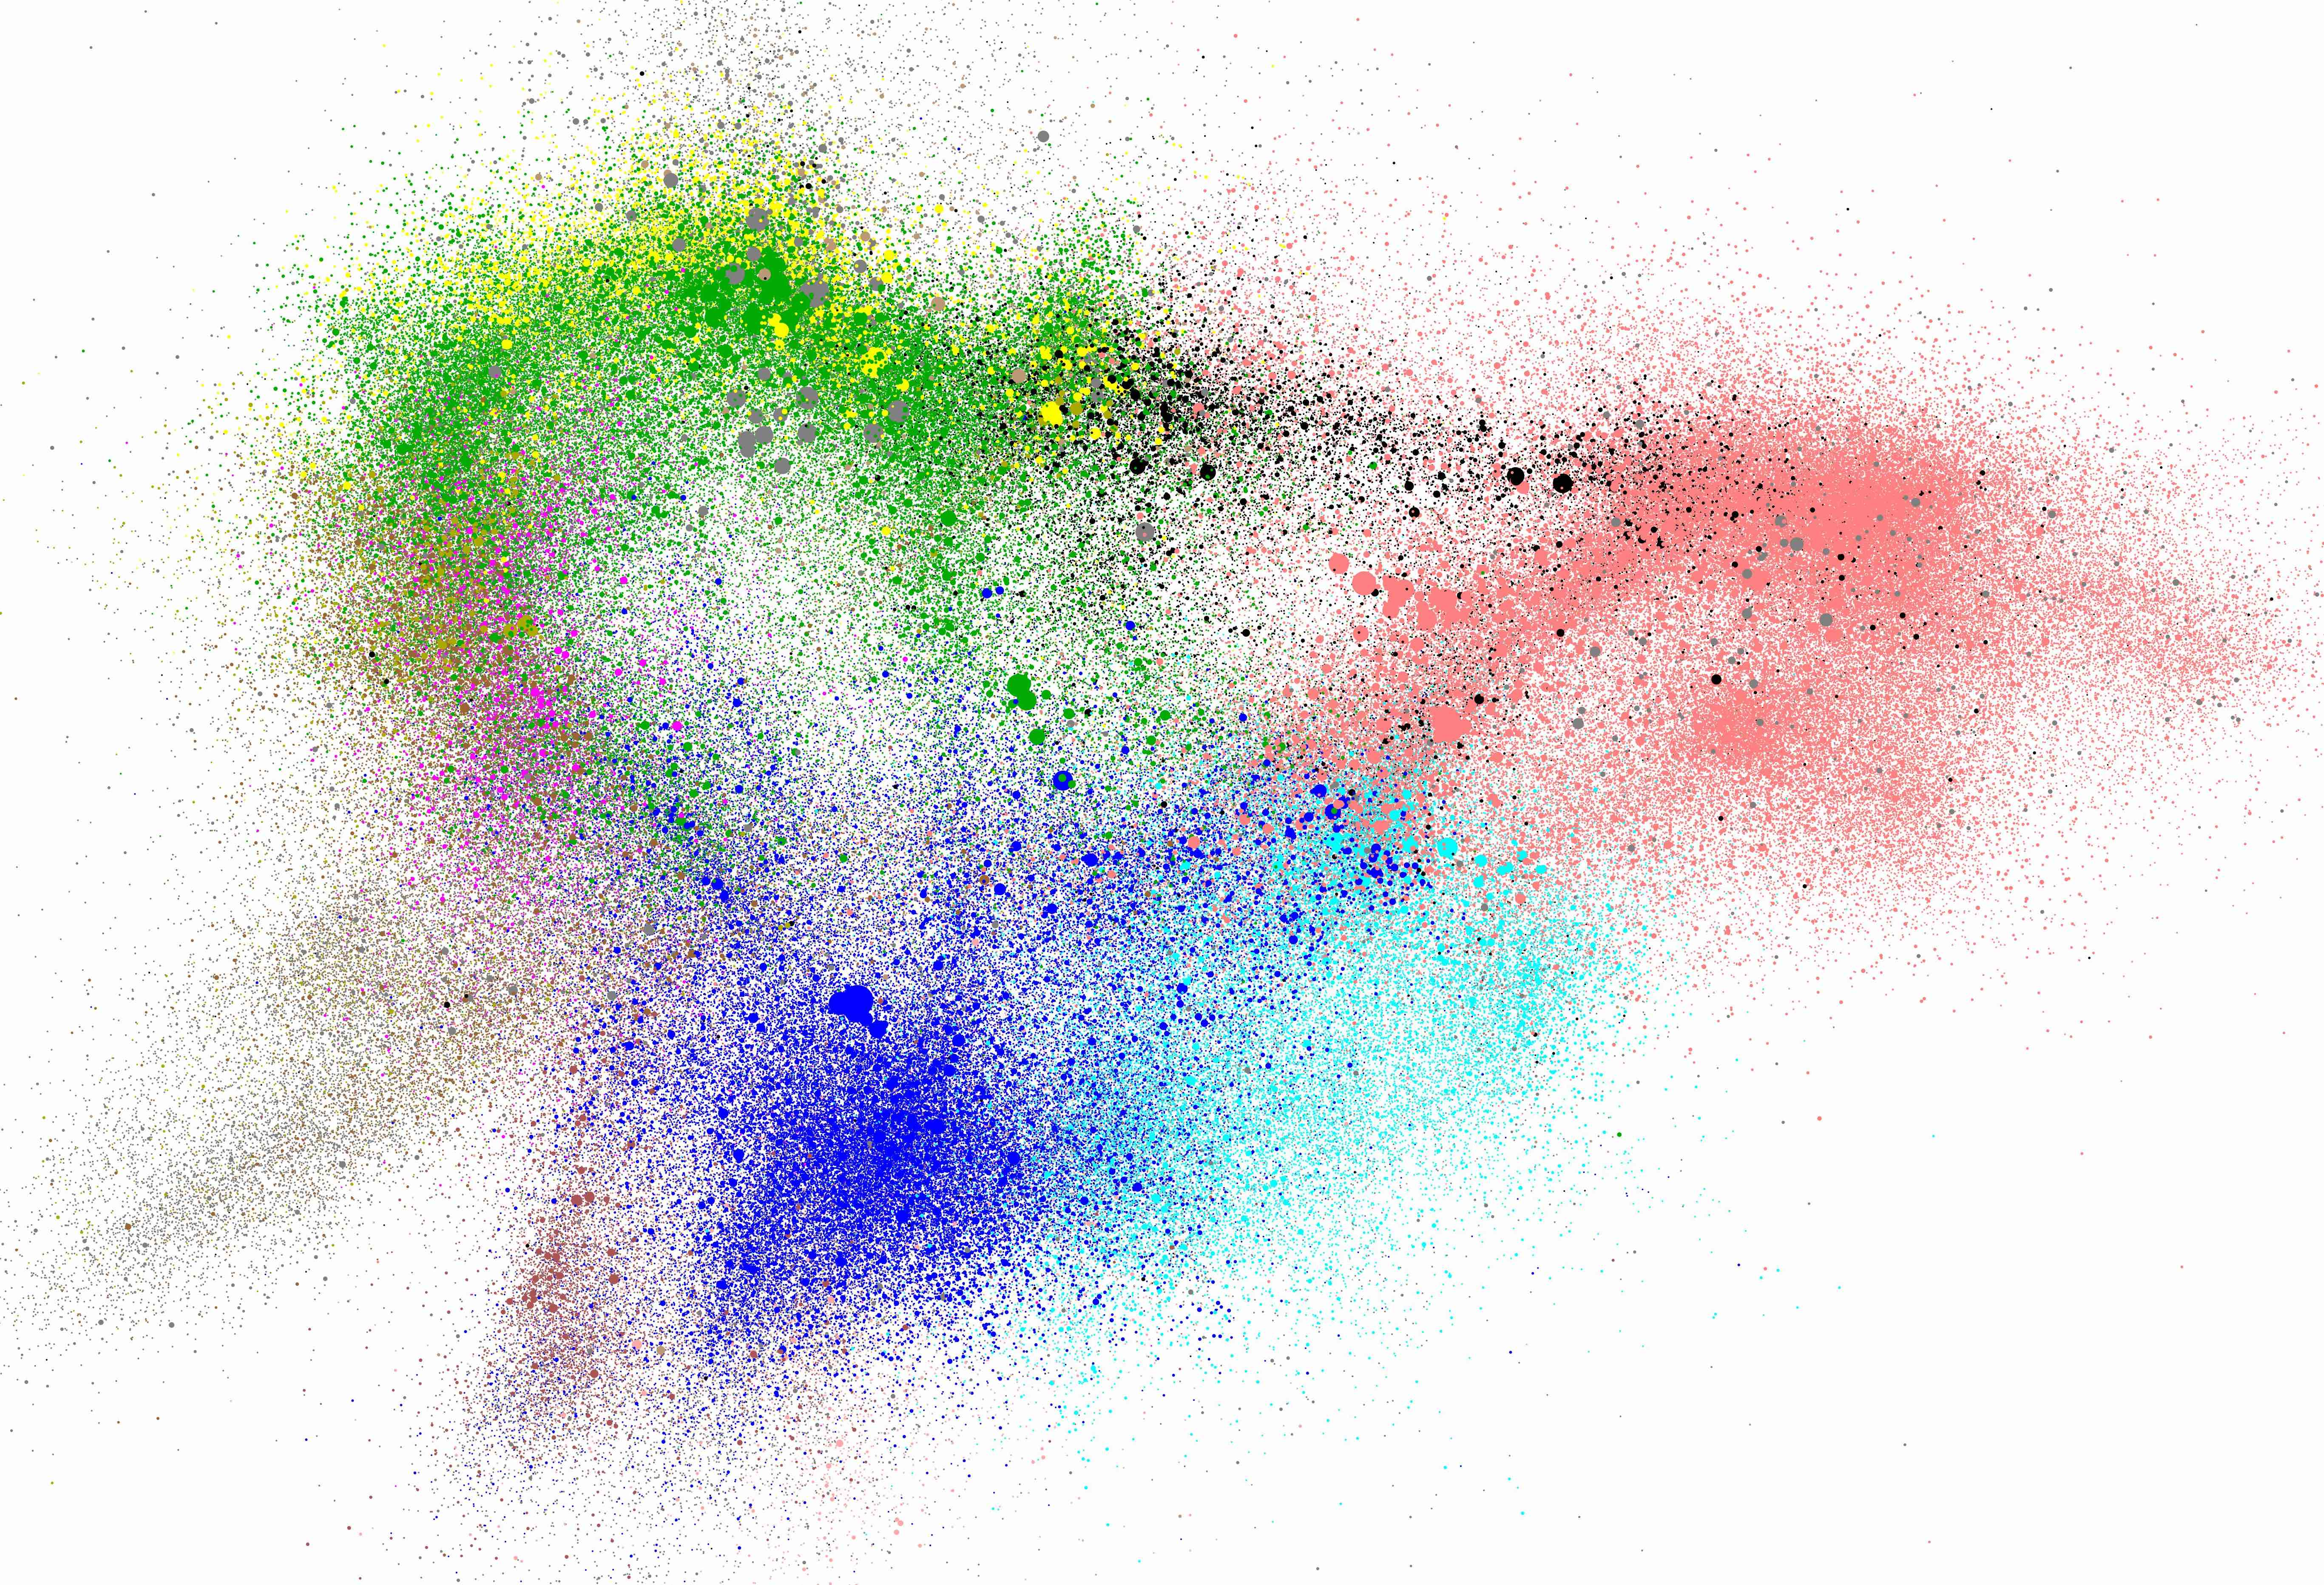
\includegraphics[width=0.9\textwidth,height=0.43\textheight]{figs/PaperScapeMyDM2022}$$
\vspace{-1ex}
\caption[DM literature]{\em 
Each dot is a paper (as extracted from the {\sc InSpire} database~\cite{InSpire} during 2022),
with size proportional to its  number of received citations,
positioned such that papers that cite each other are nearby, 
and colored according to its arXiv bulletin: 
{\color{verdes}hep-ph}, {\color{red}astro-ph}, {\color{blue}hep-th},
{\color{cyan}gr-qc}, {\color{yellow}hep-ex}, {\color{brown}nucl-th},
{\color{magenta}hep-lat}, etc.  
Papers with `dark matter' in the title 
are in black and lie at the interface between experiment, phenomenology and astrophysics.
Most other papers are unrelated to dark matter.
 \label{fig:DMpapers}  }
\end{figure}


This review is structured as follows:
\begin{itemize}
\item Part I reviews basic facts and ideas.
\begin{itemize}
\item Chapter~\ref{sec:evidences} summarizes evidence for DM from astrophysics and cosmology,
implications for its properties, and possible alternatives.

\item Chapter~\ref{chapter:distribution} summarizes what we know about the DM density and velocity distribution in the Milky Way and beyond; this will be used to compute possible DM signals.

\item Chapter~\ref{paradigms} reviews main ideas about what DM could be, from particles to waves to
primordial black holes.






\item Chapter~\ref{chapter:production} summarizes ideas about how DM formed in cosmology:
as a thermal relic, as a non-thermal relic, from inflation, etcetera.
\end{itemize}
\item Part II deals with searches for DM.
\begin{itemize}
\item Chapter~\ref{chapter:direct} reviews direct detection (DM collisions with SM particles).
\item Chapter~\ref{chapter:indirect} reviews indirect detection (DM annihilations or decays into SM particles).
\item Chapter~\ref{chapter:collider} reviews collider searches (DM production from collisions of SM particles).
\item Each chapter presents a summary of the present status in the different kinds of searches: DM has not been discovered yet, and limits are imposed. 
Then Chapter~\ref{chapter:anomalies} reviews current anomalies that might be due to DM.
While none looks compelling at present, at least they provide concrete examples of what searches mean in practice.
Many expeditions failed to reach the Poles, paving the road for the ones that eventually succeeded.

\end{itemize}
\item Part III reviews DM theories. 
\begin{itemize}
\item Chapters~\ref{models} discusses basic models of DM.
\item Chapter~\ref{BigDMtheories} discusses wider theoretical frameworks
that include possible DM candidates: super-symmetry, extra dimensions, axions\ldots
\item Alternatives to DM and their underlying theoretical frameworks are discussed in the final chapter~\ref{sec:MOND}.
\end{itemize}
\end{itemize}

%\newpage

\small
\paragraph{Acknowledgments.}
We thank, for useful discussions and information over many years, 
Asimina Arvanitaki, Shyam Balaji, Daniele Barducci,
Zurab Berezhiani, Denis Bernard, Aryaman Bhutani, Michael Blanton, Albert Bosma, Mathieu Boudaud, Giorgio Busoni,
Sandrine Codis, Paschal Coyle, Davide D'Angelo, Antonella Del Rosso, Pedro De La Torre Luque, Alo\"ise Dijoux, Caterina Doglioni, Fiorenza Donato, David Dunsky, 
Roberto Franceschini, Davide Franco, Raghuveer Garani,
Yoann G\'enolini, Gerry Gilmore, Ga\"elle Giesen, Andreas Goudelis, Benjamin Grinstein, Christian Gross, 
Keisuke Harigaya, Roni Harnik, Sebastian Hoof, Yonathan Kahn, Bradley Kavanagh, Jordan Koechler,
Fabio Iocco, Massimiliano Lattanzi, Federico Lelli, Luka Leskovec, Luca di Luzio,
Reina Maruyama, David Maurin, M.~Nicola Mazziotta, Andrea Mitridate, Emmanuel Moulin, 
Paolo Panci, Duccio Pappadopulo, Marta Perego, Federica Petricca, Elena Pinetti, Liberato Pizza,
Michele Redi,  Massimo Ricotti, Dean Robinson, Nicholas Rodd, Nicola Rossi, 
Akash Kumar Saha, Filippo Sala, Joe Silk, Francesco Sannino, Tracy Slatyer, 
Marco Taoso, Diego Tonelli, Riccardo Torre, 
Alfredo Urbano, Natascia Vignaroli, Edoardo Vitagliano, Marta Volonteri, 
Andreas Weiler, Rohana Wijewardhana, Andrea Wulzer, Wei Xue, Gabrijela Zaharijas. 
We are also particularly grateful to all our other collaborators, since some of our recent papers arose as pieces of this review that needed original work.

We also thank, for useful additional input: Kensuke Akita, Dorian Amaral, Kazem Azizi, Torsten Bringmann, Francesca Calore, Marco Chianese, Bibhabasu De, Olivier Deligny, Mattia Di Mauro, Christopher Eckner, Andrei Egorov, Astrid Eichhorn, Matteo Fasiello, Anupam Ghosh, Sergei Gninenko, Jan Heisig, Gonzalo Herrera, Mark Hertzberg, Mudit Jain, Adil Jueid, Pyungwon Ko, Silvia Manconi, Doddy Marsh, Rahul Mehra, Maurizio Piai, Nirmal Raj, Subir Sarkar, Margherita Scuderi, Robert Shrock, Jing Shu, Jusak Tandean, Edoardo Vitagliano, Jenny Wagner, Tao Xu, Wen Yin, Miguel Yulo, Michael Zantedeschi.

\medskip

The work of M.C. was supported in part by the {\em European Research Council} ({\sc Erc}) under the EU Seventh Framework Programme (FP7/2007-2013) / {\sc Erc} Starting Grant (agreement n. 278234 - `{\sc NewDark}' project) and by a {\sc Cnrs 80|Prime} grant (`{\sc DaMeFer}' project).
M.C.~acknowledges the hospitality of the {\em Institut d'Astrophysique de Paris} ({\sc Iap}), the Theory Department of {\sc Cern} and of the Physics Department of the University of California at Irvine ({\sc Uci}) where parts of this work were done. 
The work by A.S.\ has been supported by the {\sc Neo-Nat Erc} and {\sc Prin 2017fmjfmw} grants. JZ acknowledges support in part by the {\sc Doe} grant {\sc De-Sc1019775} and {\sc NSF OAC-2103889}. JZ acknowledges support in part by the Miller Institute for Basic Research in Science, University of California Berkeley.


